%!TEX program = xelatex
\documentclass[tikz]{standalone}
\usepackage{ctex}
\usepackage{fontawesome}
\usepackage{tikz}
\usepackage{epstopdf}
\usetikzlibrary{arrows,decorations.markings}
\usetikzlibrary{decorations.pathreplacing}
\usetikzlibrary{calc}
\definecolor{babypink}{rgb}{0.96, 0.76, 0.76}
\definecolor{babyblue}{rgb}{0.54, 0.81, 0.94}
\definecolor{cadmiumgreen}{rgb}{0.0, 0.42, 0.24}

\begin{document}

  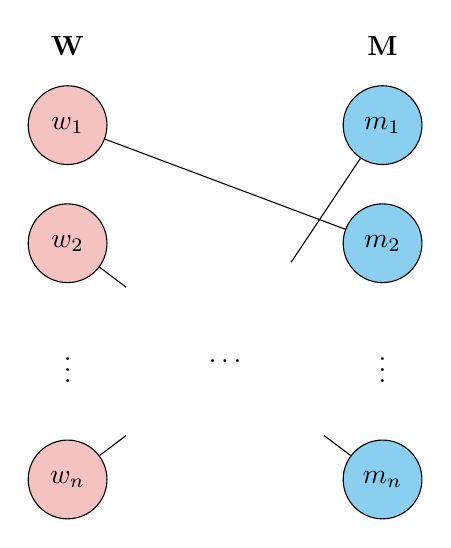
\begin{tikzpicture}[decoration={
      markings,
      mark=at position 1 with {\arrow[scale=1]{angle 90}};
    }]
    \path (0,1) node {$\mathbf{W}$};
\node[circle,draw,fill=babypink,minimum size=1cm] (w1) at (0,0) {$w_1$};
\node[circle,draw,fill=babypink,minimum size=1cm] (w2) at (0,-1.5) {$w_2$};
\path (0,-3) node {$ \vdots $};
\node[circle,draw,fill=babypink,minimum size=1cm] (wn) at (0,-4.5) {$w_n$};


\path (4,1) node {$\mathbf{M}$};
\node[circle,draw,fill=babyblue,minimum size=1cm] (m1) at (4,0) {$m_1$};
\node[circle,draw,fill=babyblue,minimum size=1cm] (m2) at (4,-1.5) {$m_2$};
\path (4,-3) node {$ \vdots $};
\node[circle,draw,fill=babyblue,minimum size=1cm] (mn) at (4,-4.5) {$m_n$};
\node[rectangle,minimum size=2.5cm] (c) at (2,-3) {$\ldots$};

\draw (w1)--(m2);
\draw (w2)--(c);
\draw (m1)--(c);
\draw (wn)--(c);
\draw (mn)--(c);

  \end{tikzpicture}

  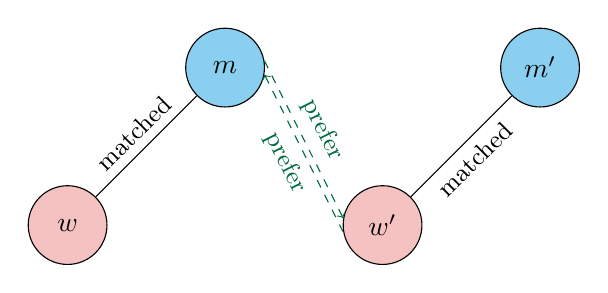
\begin{tikzpicture}[decoration={markings,
      mark=at position 1 with {\arrow[scale=1]{angle 90}};
    }]

    \node[circle,draw,fill=babypink,minimum size=1cm] (w1) at (0,0) {$w$};
\node[circle,draw,fill=babyblue,minimum size=1cm] (m1) at (2,2) {$m$};
\node[circle,draw,fill=babypink,minimum size=1cm] (w2) at (4,0) {$w'$};
\node[circle,draw,fill=babyblue,minimum size=1cm] (m2) at (6,2) {$m'$};
\draw (w1) -- node[sloped,above]{\small matched} (m1) ;
\draw (w2) -- node[sloped,below]{\small matched} (m2) ;
\draw[dashed,color=cadmiumgreen,->] (m1.10) --node[sloped,above]{\small prefer} (w2.170);
\draw[dashed,color=cadmiumgreen,->] (w2.190) --node[sloped,below]{\small prefer} (m1.350);


  \end{tikzpicture}

  \begin{tikzpicture}
    [decoration={markings,mark=at position 1 with {\arrow[scale=1]{angle 90}};}]

    \node[circle,draw,fill=babyblue,minimum size=1cm] (m) at (2,0) {$m_i$};

\node[circle,draw,fill=babypink,minimum size=1cm] (w1) at (0,2) {$w_1^i$};
\node[circle,draw,fill=babypink,minimum size=1cm] (w2) at (2,2) {$w_2^i$};
\node[circle,draw,fill=babypink,minimum size=1cm] (w3) at (4,2) {$w_3^i$};
\path (6,2) node {$\cdots$};
\node[circle,draw,fill=babypink,minimum size=1cm] (wn) at (8,2) {$w_n^i$};

\node (p1) at (0,0) {};
\node (p3) at (4,0) {};
\node (pn) at (8,0) {};

\draw[<-,color=cadmiumgreen,thick] (0,3) -- node[above]{\small prefer} (8,3);

\draw[->,thick] (m) -- node[below,align=center]{\small propose} (9,0);
\draw[<->,dashed] (w2) -- (m);
\draw[<->,dashed] (w3) -- (p3);
\draw[<->,dashed] (wn) -- (pn);
\draw[->,red,thick] (m) --node[below]{\small never back} (p1);

\path (1,0) node[color=red]{\faClose};

  \end{tikzpicture}

  \begin{tikzpicture}
    [decoration={markings,mark=at position 1 with {\arrow[scale=1]{angle 90}};}]

    \node[circle,draw,fill=babyblue,minimum size=1cm] (m1) at (6,0) {$m$};
\node[circle,draw,fill=babypink,minimum size=1cm] (w) at (3,0) {$w$};
\node[circle,draw,fill=babyblue,minimum size=1cm] (m2) at (3,3) {$m'$};


\draw[-] (m1) -- node[below]{\small match} (w);
\draw[color=cadmiumgreen,->] (m2) -- node[above,sloped]{\small propose} (w);
\draw[<->,dashed] (m1)--node[above,sloped]{\small{\textcolor{red}{$w$}} compares $\to$ responds}(m2);

\node[circle,draw,fill=babyblue,minimum size=1cm] (m3) at (14,0) {$m$};
\node[circle,draw,fill=babypink,minimum size=1cm] (w1) at (10,0) {$w$};
\node[circle,draw,fill=babyblue,minimum size=1cm] (m4) at (10,3) {$m'$};

\draw[->] (w1) --node[above,sloped]{\small accept} (m4);
\draw[-,red,dashed] (w1)--node[below]{\small break} (m3);
\path (12,0) node[red]{\faClose};

\node[circle,draw,fill=babyblue,minimum size=1cm] (m5) at (-1,0) {$m$};
\node[circle,draw,fill=babypink,minimum size=1cm] (w2) at (-4,0) {$w$};
\node[circle,draw,fill=babyblue,minimum size=1cm] (m6) at (-4,3) {$m'$};

\draw[->,dashed,red] (w2) --node[above,sloped]{\small reject} (m6);
\draw[-] (m5) -- node[below]{\small match} (w2);
\path (-4,1.5) node[red]{\faClose};

\draw[->,thick] (2,1.5) --node[above]{\small {\textcolor{red}{$w$}} prefers $m$} (-1.5,1.5);
\draw[->,thick,color=cadmiumgreen] (6,1.5) --node[above]{\small {\textcolor{red}{$w$}} prefers $m'$} (9,1.5);

  \end{tikzpicture}

  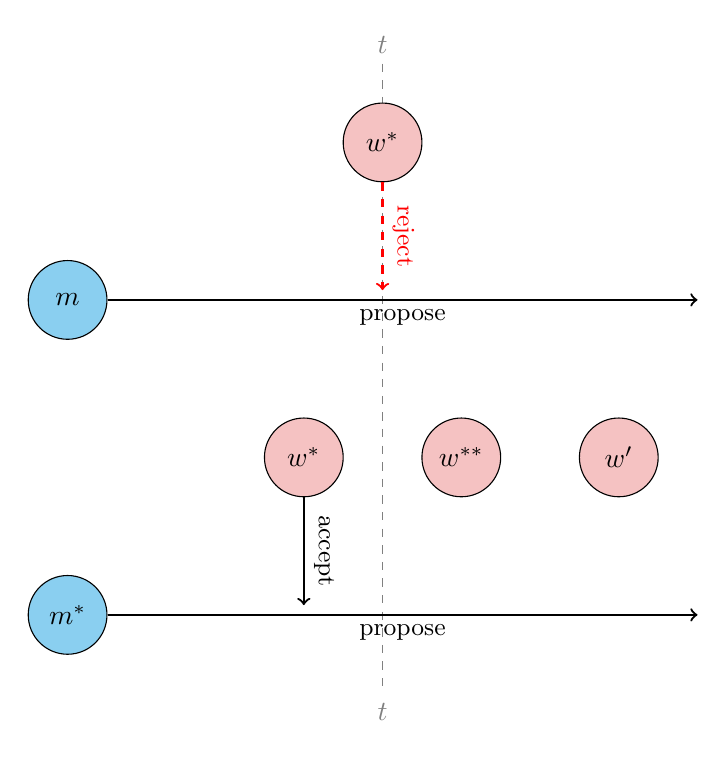
\begin{tikzpicture}
    [decoration={markings,mark=at position 1 with {\arrow[scale=1]{angle 90}};}]

    \draw[dashed,gray] (4,3) node[above]{$t$} -- (4,-5) node[below]{$t$};

\node[circle,draw,fill=babyblue,minimum size=1cm] (m1) at (0,0) {$m$};
\node[circle,draw,fill=babypink,minimum size=1cm] (w1) at (4,2) {$w^*$};
\node[circle,draw,fill=babypink,minimum size=1cm] (w2) at (3,-2) {$w^*$};
\node[circle,draw,fill=babypink,minimum size=1cm] (w3) at (5,-2) {$w^{**}$};
\node[circle,draw,fill=babypink,minimum size=1cm] (w4) at (7,-2) {$w'$};

\node[circle,draw,fill=babyblue,minimum size=1cm] (m2) at (0,-4) {$m^*$};
\node (p1) at (4,0) {};
\node (p2) at (3,-4) {};

\draw[->,thick] (m1) --node[below]{\small propose} (8,0);
\draw[->,thick] (m2) --node[below]{\small propose} (8,-4);
\draw[->,dashed,red,thick] (w1) -- node[sloped,above]{\small reject} (p1);

\draw[->,thick] (w2) -- node[sloped,above]{\small accept} (p2);

  \end{tikzpicture}

  \begin{tikzpicture}
    [decoration={markings,mark=at position 1 with {\arrow[scale=1]{angle 90}};}]

    \draw[dashed,opacity=0.7,color=babyblue] (-2,2) -- (6,2);
\draw[dashed,opacity=0.7,color=babyblue] (-2,4) -- (6,4);
\draw[dashed,opacity=0.7,color=babypink] (-2,0) -- (6,0);
\draw[dashed,opacity=0.7,color=babypink] (-2,-2) -- (6,-2);



\node[circle,draw,fill=babyblue,minimum size=1cm] (m1) at (0,4) {$m$};
\node[circle,draw,fill=babypink,minimum size=1cm] (w1) at (5,0) {$w$};
\node[circle,draw,fill=babyblue,minimum size=1cm] (m2) at (5,2) {$m'$};
\node[circle,draw,fill=babypink,minimum size=1cm] (w2) at (0,-2) {$w'$};

\draw[thick] (w2)-- node[above,sloped]{\footnotesize matched in $S$}(m1);
\draw[thick] (w1)-- node[below,sloped,yshift=-0.5cm]{\footnotesize matched in $S$}(m2);

\draw [decorate,decoration={brace,amplitude=10pt,mirror,raise=2pt}]
(5.5,2) -- node[midway,right,xshift=0.4cm]{\small {\color{babypink}{$w$}} prefers ${\color{babyblue}{m}}>{\color{babyblue}{m'}}$} (5.5,4);

\draw [decorate,decoration={brace,amplitude=10pt,raise=2pt}]
(-0.5,-2) -- node[midway,left,xshift=-0.4cm]{\small ${\color{babyblue}{m}}$ prefers ${\color{babypink}{w}}>{\color{babypink}{w'}}$} (-0.5,0);

\draw[thick,dashed,red] (w1) --node[sloped]{\Large\faExclamationTriangle} (m1);

  \end{tikzpicture}

  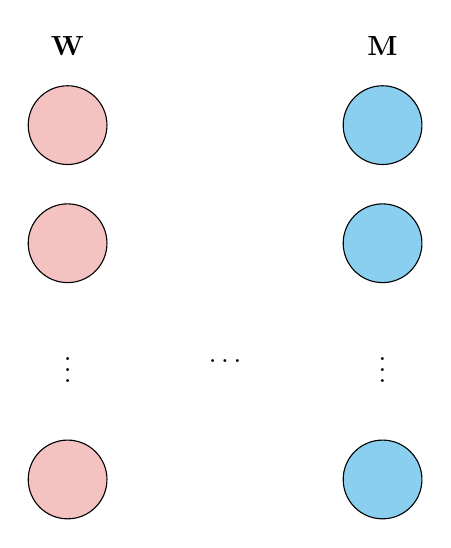
\begin{tikzpicture}
    [decoration={markings,mark=at position 1 with {\arrow[scale=1]{angle 90}};}]

    \path (0,1) node {$\mathbf{W}$};
\node[circle,draw,fill=babypink,minimum size=1cm] (w1) at (0,0) {};
\node[circle,draw,fill=babypink,minimum size=1cm] (w2) at (0,-1.5) {};
\path (0,-3) node {$ \vdots $};
\node[circle,draw,fill=babypink,minimum size=1cm] (wn) at (0,-4.5) {};

\path (4,1) node {$\mathbf{M}$};
\node[circle,draw,fill=babyblue,minimum size=1cm] (m1) at (4,0) {};
\node[circle,draw,fill=babyblue,minimum size=1cm] (m2) at (4,-1.5) {};
\path (4,-3) node {$ \vdots $};
\node[circle,draw,fill=babyblue,minimum size=1cm] (mn) at (4,-4.5) {};
\node[rectangle,minimum size=2.5cm] (c) at (2,-3) {$\ldots$};

  \end{tikzpicture}



\end{document}
